\chapter{Parametric Inference}

\begin{ex}
  Recall that if $X\sim\text{Gamma}(\alpha,\beta)$, then by Exercise 3.12,
  \[
    \E{X}=\alpha\beta,\quad
    \E{X^2} =\alpha(\alpha+1)\beta^2
    =(\alpha\beta)^2+(\alpha\beta)\beta.
  \]
  Recall that $\alphahat_1=\frac{1}{n}\sum_{i=1}^n X_i$ and
  $\alphahat_2=\frac{1}{n}\sum_{i=1}^n X_i^2$. Then,
  \[
    \begin{cases}
      \alphahat_1 = \alphahat\betahat \\
      s = \alphahat_1^2+\alphahat_1\betahat
    \end{cases} \implies
    \begin{cases}
      \alphahat_1 = \alphahat\betahat \\
      \betahat = (\alphahat_2 - \alphahat_1^2)/\alphahat_1
    \end{cases} \implies
    \begin{cases}
      \alphahat = \alphahat_1^2/(\alphahat_2-\alphahat_1^2) \\
      \betahat = (\alphahat_2-\alphahat_1^2)/\alphahat_1
    \end{cases}.
  \]
\end{ex}

\begin{ex}~
  \begin{enumerate}[(a)]
    \item Recall that if $X\sim\text{Uniform}(a, b)$,
          \[
            \E{X}=(a+b)/2,\text{ and } \E{X^2}=\var{X}+\E{X}^2=(a^2+ab+b^2)/3.
          \]
          Then,
          \begin{align*}
            \begin{cases}
              \alphahat_1 = (\ahat + \bhat)/2                 \\
              \alphahat_2 = (\ahat^2 + \ahat\bhat +\bhat^2)/3 \\
            \end{cases}\implies
            \begin{cases}
              2\alphahat_1 - \ahat = \bhat              \\
              4\alphahat_1^2 -3\alphahat_2 = \ahat\bhat \\
            \end{cases}\implies
            \begin{cases}
              2\alphahat_1 - \ahat = \bhat                            \\
              \ahat^2-2\alphahat_1\ahat+4\alphahat_1^2-3\alphahat_2=0 \\
            \end{cases},
          \end{align*}
          or solving the quadratic equation,
          \[
            \ahat=\alphahat_1\pm \sqrt{3}\sqrt{\alphahat_2-\alphahat_1^2}.
          \]
          Note that then $\bhat$ is the other solution to the quadratic
          equation, and, since $b\geq a$, we have
          \[
            \ahat=\alphahat_1- \sqrt{3}\sqrt{\alphahat_2-\alphahat_1^2},
            \quad
            \bhat=\alphahat_1+ \sqrt{3}\sqrt{\alphahat_2-\alphahat_1^2}.
          \]
    \item Let $\theta=(a,b)$. Note that then
          \[
            \L_n(\theta)=\prod_{i=1}^n \frac{I_{[a, b]}(x_i)}{b-a}
            =\begin{cases}
              (b-a)^{-n} & \text{$x_i\in [a, b]$ for all $i$}, \\
              0          & \text{otherwise}.
            \end{cases}
          \]
          Thus, to maximize $\L_n(\theta)$, we must have $a\leq X_{(1)}$ and
          $b\geq X_{(n)}$. Moreover, note that $\L_n(\theta)$ increases as $b$
          increases, and decreases as $a$ increases. Therefore,
          $\ahat= X_{(1)}$ and $\bhat= X_{(n)}$.
    \item Let $\theta=(a, b)$. Note that then
          $\tau(\theta)=\int\!x\,\d{F}(x)=\E{X}=(a+b)/2$. However, by the
          equivariance of the maximum likelihood estimator, $\tauhat
            =g(\thetahat)=(X_{(1)}+X_{(n)})/2$.
    \item Recall that the plug-in estimator of the mean is given by the sample
          average and that, by Example 7.10,
          \[
            \E{\widetilde{\tau}}   = (a + b) / 2,\quad
            \var{\widetilde{\tau}} = \frac{\sigma^2_X}{n}
            =\frac{1}{n}\frac{(b-a)^2}{12}.
          \]
          Hence,
          \[
            \mse{\tauhat}
            =\bias{\tauhat}^2
            +\var{\tauhat}
            =\frac{1}{n}\frac{(b-a)^2}{12}.
          \]
          \inputminted{python}{../code/09-02.py}
          \inputminted{text}{../output/09-02.txt}
  \end{enumerate}
\end{ex}

\begin{ex}~
  \begin{enumerate}[(a)]
    \item Let $X\sim N(\mu,\sigma^2)$. Then
          \[
            0.95
            =\P{X<\tau}
            =\P{\frac{X-\mu}{\sigma}<\frac{\tau-\mu}{\sigma}}
            =\Phi\left(\frac{\tau-\mu}{\sigma} \right),
          \]
          or,
          \[
            \tau=\Phi^{-1}(0.95)\sigma+\mu.
          \]

          Recall that by Example 9.11, the maximum likelihood estimators for $X$
          are
          \[
            \muhat = \Xbar,\text{ and }
            \sigmahat = S,
          \]
          and that therefore by the equivariance of the MLE,
          \[
            \widehat{\tau}=1.645\cdot S+\Xbar.
          \]
    \item We will use the delta method. Note that by Exercise 9.8,
          \[
            I_n(\mu,\sigma)
            =\begin{pmatrix}
              \frac{n}{\sigma^2} & 0                   \\
              0                  & \frac{2n}{\sigma^2}
            \end{pmatrix},
          \]
          and that therefore
          \[
            J_n=I^{-1}_n(\mu,\sigma)
            =\frac{1}{n}\begin{pmatrix}
              \sigma^2 & 0                  \\
              0        & \frac{\sigma^2}{2}
            \end{pmatrix}.
          \]
          Let $g(\mu,\sigma)=1.645 \sigma+\mu$. Note that
          $\nabla g=(1, 1.645)$, and that therefore
          \begin{align*}
            \widehat{\textsf{se}}(\widehat{\tau})
             & =\sqrt{\begin{pmatrix}
                1 & 1.645 \\
              \end{pmatrix}
              \begin{pmatrix}
                \sigmahat^2 & 0                     \\
                0           & \frac{\sigmahat^2}{2}
              \end{pmatrix}
              \begin{pmatrix}
                1 \\ 1.645
              \end{pmatrix}}
            =\frac{1.534\sigmahat}{\sqrt{n}}.
          \end{align*}

          Therefore,
          \[
            C_n=\left(
            1.645\cdot S+\Xbar-z_{\alpha/2}\frac{1.534 S}{\sqrt{n}},
            1.645\cdot S+\Xbar+z_{\alpha/2}\frac{1.534 S}{\sqrt{n}}
            \right).
          \]
    \item~
          \inputminted{python}{../code/09-03.py}
          \inputminted{text}{../output/09-03.txt}
  \end{enumerate}
\end{ex}

\begin{ex}
  Let $X_1,\ldots,X_n\sim\text{Uniform}(0,\theta)$. Recall that the maximum
  likelihood estimator for $\theta$ is given by the maximum of the examples, and
  that therefore, for $0<\epsilon<\theta$,
  \begin{align*}
    \P{\left|\widehat{\theta}_n-\theta\right|>\epsilon}
     & =\P{\widehat{\theta}_n < \theta-\epsilon}                 \\
     & =\P{X_1 < \theta-\epsilon}\cdots\P{X_n < \theta-\epsilon} \\
     & =\left(\frac{\theta-\epsilon}{\theta}\right)^n            \\
     & =\left(1-\frac{\epsilon}{\theta}\right)^n
  \end{align*}
  which goes to $0$ as $n$ goes to infinity. Hence,
  $\widehat{\theta}_n\xrightarrow{P} \theta$, and therefore the maximum
  likelihood estimator is consistent.
\end{ex}

% 5
\begin{ex}
  Let $X\sim\text{Poisson}(\lambda)$. Recall that then
  \[
    f_X(x)=\frac{\lambda^x e^{-\lambda}}{x!},
  \]
  and that
  \[
    \E{X}
    =\sum_{x=0}^\infty x\frac{\lambda^x e^{-\lambda}}{x!}
    =\lambda\sum_{x=1}^\infty \frac{\lambda^{x-1} e^{-\lambda}}{(x-1)!}
    =\lambda.
  \]
  Hence, the method of moments estimator for $\lambda$ is given by $\Xbar$.

  Note that
  \[
    \ell(\lambda)
    =\log\left(\frac{\lambda^X e^{-\lambda}}{X!}\right)
    =X\log{\lambda}-\lambda-\log{X!},
  \]
  and that therefore
  \[
    \frac{\pd}{\pd\lambda}\ell(\lambda)
    =X/\lambda-1.
  \]
  Hence,
  \[
    0=\ell_n(\lambda)=\sum_{i=1}^n(X_i/\lambda -1)
  \]
  implies that
  \[
    n=(n/\lambda)\Xbar
  \]
  or
  \[
    \lambda=\Xbar.
  \]
  This is a maximum since the second derivative is negative. Hence,
  $\widehat{\lambda}=\Xbar$.

  Finally, note that
  \[
    I(\lambda)=-\E{\frac{\pd^2}{\pd\lambda^2}\ell(\lambda)}
    =-\E{-X/\lambda^2}=\lambda^{-1}.
  \]
\end{ex}

\begin{ex}~
  \begin{enumerate}[(a)]
    \item We have
          \[
            \psi=\P{Y_1=1}=\P{X_1>0}=\P{X_1-\theta>-\theta}=1-\Phi(-\theta)
            =\Phi(\theta).
          \]
          Recall that the maximum likelihood estimator for $\theta$ is
          $\overline{X}=\frac{1}{n}\sum_{i=1}^nX_i$. Therefore, by the
          equivariance of the maximum likelihood, it follows that
          $\widehat{\psi}=\Phi(\overline{X})$.
    \item We will use the delta method. Note that
          $\psi=g(\theta)=\Phi(\theta)$, and that therefore
          $g'(\theta)=\phi(\theta)$. By Exercise 9.8, $I_n(\theta)=n$, and
          thus $\widehat{\textsf{se}}(\widehat{\theta})=\sqrt{1/n}$. Hence,
          \[
            \widehat{\textsf{se}}(\widehat{\psi})=\phi(\overline{X})/\sqrt{n}.
          \]
          Therefore, a $95\%$ confidence interval for $\psi$ is
          \[
            C_n=\left(
            \Phi(\overline{X})-z_{0.05/2}\phi(\overline{X})/\sqrt{n},
            \Phi(\overline{X})+z_{0.05/2}\phi(\overline{X})/\sqrt{n}
            \right).
          \]
    \item Since $\E{Y_i}=\P{Y_i=1}=\P{Y_1=1}=\psi$, and $\psihat$ is an
          average of $Y_i$'s, the result follows by the law of large numbers.
    \item We have
          \[
            \var{\psihat}
            =\var{\frac{1}{n}\sum_{i=1}^n Y_i}
            =\frac{1}{n^2}\sum_{i=1}^n \var{Y_i}
            =\frac{\Phi(\theta)(1-\Phi(\theta))}{n}.
          \]
          Thus,
          \[
            \textsc{are}(\widehat{\psi},\widetilde{\psi})
            =
            \frac{\var{\widetilde{\psi}}}{\var{\widehat{\psi}}}
            =\frac{\Phi(\theta)(1-\Phi(\theta))}{\phi^2(\theta)}.
          \]
    \item We have that $\E{\overline{X}}=\E{X_i}=\mu_X$, and therefore
          $\widehat{\psi}$ still converges to $\Phi(\mu_X)$ by
          the law of large numbers. However, $\psi=\P{Y_1=1}=
            \P{X_i>0}=1-F_X(0)$, where
          $\Phi(\mu_X)\neq 1-F_X(0)$ for an arbitrary $F_X$.
  \end{enumerate}
\end{ex}

\begin{ex}~
  \begin{enumerate}[(a)]
    \item Let $X\sim\text{Binomial(n, p)}$. Note that then
          \[
            f_{X}(x)=\binom{n}{x}p^x(1-p)^{n-x}
          \]
          and that therefore
          \[
            \ell_X(p)=\log\left[\binom{n}{X}\right]+X\log{p}+(n-X)\log(1-p),
          \]
          and
          \[
            \frac{\pd}{\pd p}\ell(p)=X/p-(n-X)/(1-p).
          \]
          Setting $\frac{\pd}{\pd p}\ell(p)$ equal to $0$ and solving for $p$,
          we get that $\widehat{p}=X/n$ is the maximum likelihood estimator
          for a Binomial distribution.

          Next, let $X_1\sim\text{Binomial}(n_1, p_1)$ and
          $X_2\sim\text{Binomial}(n_1, p_1)$ as in the problem. Since $X_1$ and
          $X_2$ are independent, it follows that the maximum likelihood
          estimator for $(p_1,p_2)$ is $(X_1/n_1, X_2/n_2$. Hence, by the
          equivariance of the maximum likelihood estimator, since
          $\psi=g(p_1,p_2)=p_1-p_2$, $\widehat{\psi}=X_1/n_1-X_2/n_2$.
    \item The density for the joint distribution is
          \[
            f_{X_1,X_2}(x_1,x_2)=
            \left[\binom{n_1}{x_1}p_1^{x_1}(1-p_1)^{n_1-x_1}\right]
            \left[\binom{n_2}{x_2}p_2^{x_2}(1-p_2)^{n_2-x_2}\right],
          \]
          and therefore
          \begin{align*}
            \ell_{X_1,X_2}(p_1,p_2)
             & =\log\left[\binom{n_1}{X_1}\right]+X_1\log{p_1}+(n_1-X_1)\log(1-p_1)       \\
             & \quad+\log\left[\binom{n_2}{X_2}\right]+X_2\log{p_2}+(n_2-X_2)\log(1-p_2).
          \end{align*}
          Hence,
          \begin{align*}
            H_{11}
            =\frac{\pd^2 \ell_{X_1,X_2}}{\pd p_1^2}
            =-\frac{X_1}{p_1^2}-\frac{n_1-X_1}{(1-p_1)^2},
          \end{align*}
          and
          \begin{align*}
            -\E{H_{11}}
            =\frac{np_1}{p_1^2}+\frac{n_1-n_1p_1}{(1-p_1)^2}
            =\frac{n_1}{p_1}+\frac{n_1}{1-p_1}
            =\frac{n_1}{p_1(1-p_1)}.
          \end{align*}
          By symmetry, we also have
          \[
            -\E{H_{22}}
            =\frac{n_2}{p_2(1-p_2)},
          \]
          and by independence, it follows that
          \[
            H_{12}=H_{21}=0.
          \]

          Therefore,
          \begin{align*}
            I(p_1, p_2)
             & =\begin{pmatrix}
              \frac{n_1}{p_1(1-p_1)} & 0                      \\
              0                      & \frac{n_2}{p_2(1-p_2)}
            \end{pmatrix}.
          \end{align*}
    \item Recall that $\psi=g(p_1,p_2)=p_1-p_2$, and therefore
          $\nabla g=(1,-1)$. Hence, by the multiparameter delta method
          \[
            \widehat{\textsf{se}}(\widehat{\psi})
            =\sqrt{
              \begin{pmatrix}
                1 & -1
              \end{pmatrix}
              \begin{pmatrix}
                \frac{p_1(1-p_1)}{n_1} & 0                      \\
                0                      & \frac{p_2(1-p_2)}{n_2}
              \end{pmatrix}
              \begin{pmatrix}
                1 \\ -1
              \end{pmatrix}
            }
            =\sqrt{\frac{p_1(1-p_1)}{n_1} + \frac{p_2(1-p_2)}{n_2}}.
          \]
    \item
          \inputminted{python}{../code/09-07.py}
          \inputminted{text}{../output/09-07.txt}
  \end{enumerate}
\end{ex}

\begin{ex}
  Let $X\sim N(\mu,\sigma^2)$. Let $\theta=(\mu,\sigma)$. Note that then
  \[
    \ell(\theta)
    =-\frac{1}{2}\frac{(x-\mu)^2}{\sigma^2}+\log{\frac{1}{\sigma\sqrt{2\pi}}},
  \]
  and, therefore
  \[
    H_{11}
    =\frac{\pd^2\ell_n}{\pd\mu^2}
    =-\frac{n}{\sigma^2},\quad
    \E{H_{11}} =-\frac{n}{\sigma^2},
  \]
  \[
    H_{22}
    =\frac{\pd^2\ell_n}{\pd\sigma^2}
    =\frac{n}{\sigma^2}-\frac{3n(x-\mu)^2}{\sigma^4},\quad
    \E{H_{22}}=\frac{n}{\sigma^2}-\frac{3n\E{(x-\mu)^2}}{\sigma^4}
    =-\frac{2n}{\sigma^2},
  \]
  \[
    H_{12}
    =\frac{\pd^2\ell_n}{\pd\mu\pd\sigma}
    =\frac{\pd}{\pd\mu}\left[\frac{n(x-\mu)^2-n\sigma^2}{\sigma^2}\right]
    =-\frac{2n(x-\mu)}{\sigma^3},\quad
    \E{H_{12}} = 0,
  \]
  \[
    H_{21}
    =\frac{\pd^2\ell_n}{\pd\sigma\pd\mu}
    =\frac{\pd}{\pd\sigma}\left[-\frac{n(x-\mu)}{\sigma^2}\right]
    =-\frac{2n(x-\mu)}{\sigma^3},\quad
    \E{H_{21}} = 0.
  \]

  Hence,
  \[
    I_n(\mu,\sigma)
    =\begin{pmatrix}
      \frac{n}{\sigma^2} & 0                   \\
      0                  & \frac{2n}{\sigma^2}
    \end{pmatrix}.
  \]
\end{ex}

\begin{ex}~
  \begin{enumerate}[(a)]
    \item Recall that for $X_1,\ldots,X_n\sim N(0,\sigma^2)$,
          $I_n(\mu)=n/\sigma^2$, and therefore, since $g(\mu)=e^\mu$,
          $g'=e^\mu$ and by the delta method,
          \[
            \widehat{\textsf{se}}(\widehat{\theta})
            =\frac{e^{\Xbar}S}{\sqrt{n}},
          \]
          and
          \[
            C_n=\left(
            e^{\Xbar}-z_{\alpha/2}\frac{e^{\Xbar}S}{\sqrt{n}},
            e^{\Xbar}+z_{\alpha/2}\frac{e^{\Xbar}S}{\sqrt{n}}
            \right),
          \]
          is a $1-\alpha$ confidence interval for $\widehat{\theta}$.

          \inputminted{python}{../code/09-09.py}
          \inputminted{text}{../output/09-09.txt}
    \item~
          \begin{figure}[H]
            \centering
            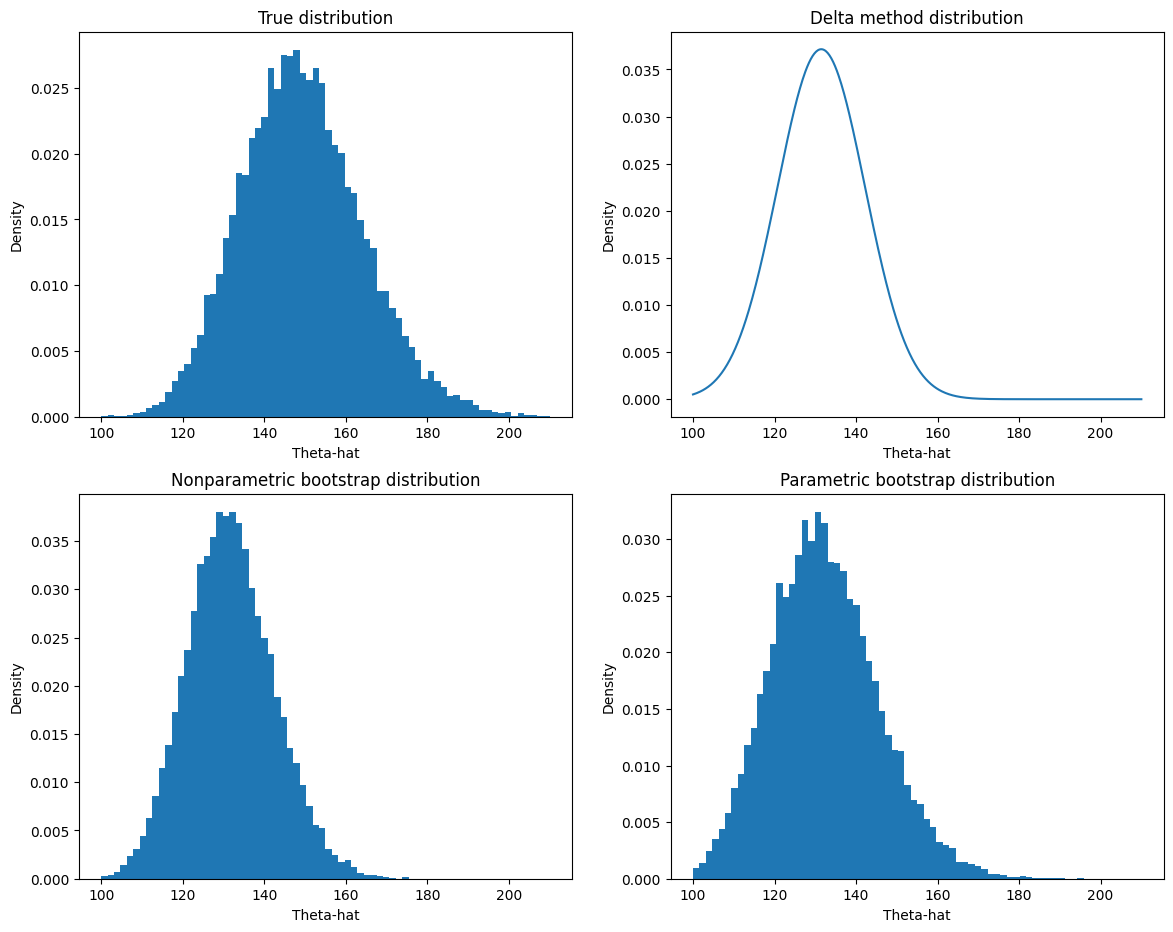
\includegraphics[scale=0.53]{../images/09-09}
            \caption{A comparison of a histogram of the true distribution of
              $\widehat{\theta}$ (upper left), non-parametric bootstrap
              replicates (lower left), parametric bootstrap replicates
              (lower right) and a plot of the delta method distribution
              (upper right).}
          \end{figure}
  \end{enumerate}
\end{ex}

\begin{ex}~
  \begin{enumerate}[(a)]
    \item We have
          \begin{align*}
            \P{\widehat{\theta}\leq x}
             & =\P{X_{(n)}\leq x}                               \\
             & =\P{X_{1}\leq x}\P{X_2\leq x}\cdots\P{X_n\leq x} \\
             & =x^n,
          \end{align*}
          and therefore
          \[
            f_{\widehat{\theta}}(x)=nx^{n-1}. \\
          \]

          \inputminted{python}{../code/09-10.py}

          \begin{figure}[H]
            \centering
            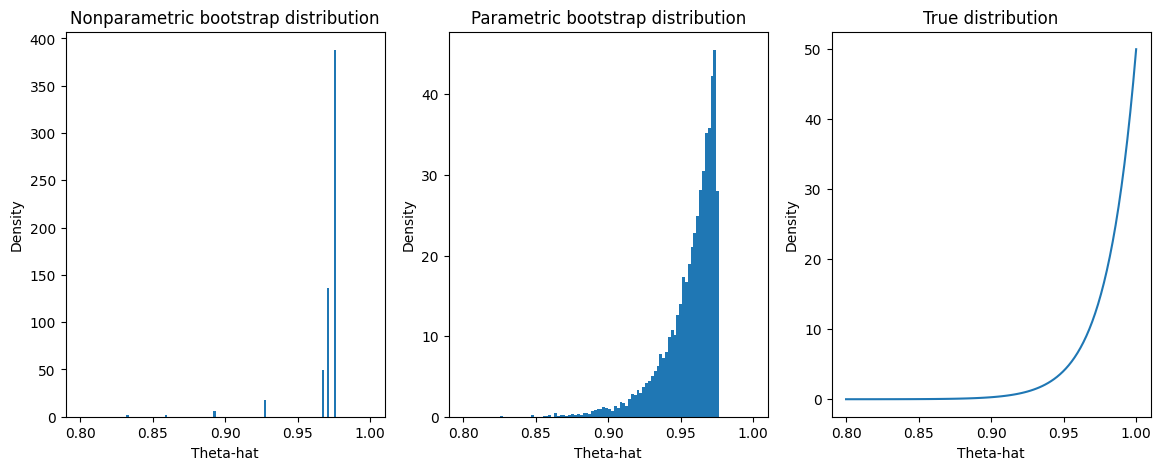
\includegraphics[scale=0.53]{../images/09-10}
            \caption{
              A comparison of a histogram of the non-parametric bootstrap
              (left), the parametric bootstrap (center) and the true
              distribution of $\widehat{\theta}$ (right).}
          \end{figure}
    \item Let $B$ be a random variable given by uniformly randomly sampling
          from $\{X_1,X_2,\ldots,X_n\}$, and let $B^n$ be a sample (with
          replacement) of $n$ elements. Then,
          \begin{align*}
            \P{\widehat{\theta}^*=\widehat{\theta}}
             & =\P{X_{(n)}\in B^n}              \\
             & =1-\P{X_{(n)}\not\in B^n}        \\
             & =1-(1-\P{B = X_{(n)}})^n         \\
             & =1-\left(1-\frac{1}{n}\right)^n,
          \end{align*}
          and therefore
          \[
            \lim_{n\to\infty}\P{\widehat{\theta}^*
              =\widehat{\theta}}
            =1-e^{-1}
            \approx 0.632.
          \]
          However, since $\widehat{\theta}$ has a continuous distribution, the
          probability that it takes on any particular value is $0$. Therefore,
          we cannot use the bootstrap to obtain an arbitrarily good
          approximation of $\widehat{\theta}$, no matter how many samples we
          use.
  \end{enumerate}
\end{ex}